% This file was created with matplot2tikz v0.5.4.
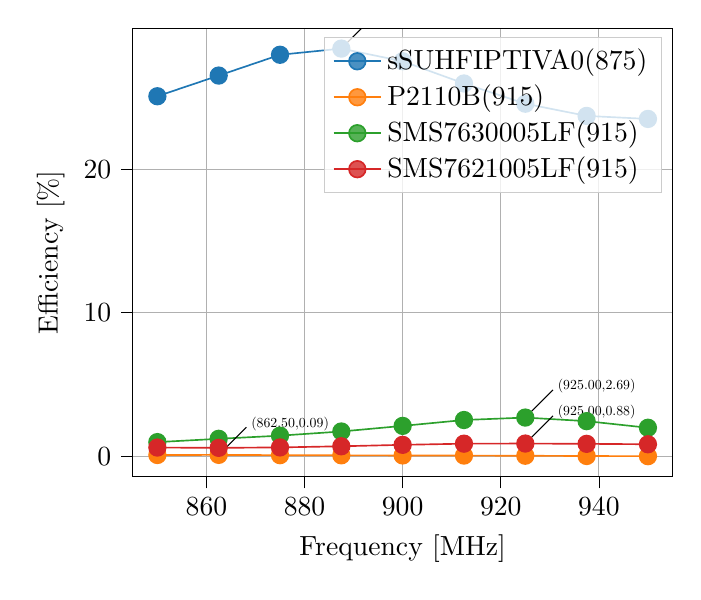
\begin{tikzpicture}

\definecolor{crimson2143940}{RGB}{214,39,40}
\definecolor{darkgray176}{RGB}{176,176,176}
\definecolor{darkorange25512714}{RGB}{255,127,14}
\definecolor{forestgreen4416044}{RGB}{44,160,44}
\definecolor{lightgray204}{RGB}{204,204,204}
\definecolor{steelblue31119180}{RGB}{31,119,180}

\begin{axis}[
legend cell align={left},
legend style={fill opacity=0.8, draw opacity=1, text opacity=1, draw=lightgray204},
tick align=outside,
tick pos=left,
x grid style={darkgray176},
xlabel={Frequency [MHz]},
xmajorgrids,
xmin=845, xmax=955,
xtick style={color=black},
y grid style={darkgray176},
ylabel={Efficiency [\%]},
ymajorgrids,
ymin=-1.42, ymax=29.82,
ytick style={color=black}
]
\addplot [semithick, steelblue31119180, mark=*, mark size=3, mark options={solid}]
table {%
850 25.08
862.5 26.52
875 27.97
887.5 28.4
900 27.52
912.5 25.97
925 24.56
937.5 23.71
950 23.5
};
\addlegendentry{sSUHFIPTIVA0(875)}
\addplot [semithick, darkorange25512714, mark=*, mark size=3, mark options={solid}]
table {%
850 0.08
862.5 0.09
875 0.07
887.5 0.06
900 0.05
912.5 0.04
925 0.03
937.5 0.01
950 0
};
\addlegendentry{P2110B(915)}
\addplot [semithick, forestgreen4416044, mark=*, mark size=3, mark options={solid}]
table {%
850 0.98
862.5 1.21
875 1.43
887.5 1.72
900 2.11
912.5 2.52
925 2.69
937.5 2.44
950 1.98
};
\addlegendentry{SMS7630005LF(915)}
\addplot [semithick, crimson2143940, mark=*, mark size=3, mark options={solid}]
table {%
850 0.6
862.5 0.58
875 0.61
887.5 0.69
900 0.79
912.5 0.87
925 0.88
937.5 0.86
950 0.83
};
\addlegendentry{SMS7621005LF(915)}
\draw[->,draw=black] (axis cs:887.5,28.4) ++(10pt,10pt) -- (axis cs:887.5,28.4);
\draw (axis cs:887.5,28.4) ++(10pt,10pt) node[
  scale=0.5,
  anchor=base west,
  text=black,
  rotate=0.0
]{(887.50,28.40)};
\draw[->,draw=black] (axis cs:862.5,0.09) ++(10pt,10pt) -- (axis cs:862.5,0.09);
\draw (axis cs:862.5,0.09) ++(10pt,10pt) node[
  scale=0.5,
  anchor=base west,
  text=black,
  rotate=0.0
]{(862.50,0.09)};
\draw[->,draw=black] (axis cs:925,2.69) ++(10pt,10pt) -- (axis cs:925,2.69);
\draw (axis cs:925,2.69) ++(10pt,10pt) node[
  scale=0.5,
  anchor=base west,
  text=black,
  rotate=0.0
]{(925.00,2.69)};
\draw[->,draw=black] (axis cs:925,0.88) ++(10pt,10pt) -- (axis cs:925,0.88);
\draw (axis cs:925,0.88) ++(10pt,10pt) node[
  scale=0.5,
  anchor=base west,
  text=black,
  rotate=0.0
]{(925.00,0.88)};
\end{axis}

\end{tikzpicture}
